% Template LaTeX document for CSSR4Africa Deliverables
% Adapted from documents prepared by EPFL for the RobotCub project
% and subsequently by the University of Skövde for the DREAM project
%
% DV 28/06/2023

\documentclass{CSSRforAfrica}

\usepackage[titletoc,title]{appendix}
\usepackage[colorlinks, urlcolor=blue, linkcolor=black, citecolor=black]{hyperref}
\usepackage{latexsym}
\usepackage{comment}
\usepackage{multirow}
\usepackage{subcaption}
\usepackage[breakable,skins,most]{tcolorbox} % Consolidated tcolorbox options
\usepackage{tabularx,colortbl}
\usepackage[tikz]{bclogo} % for boxes
\usepackage{ragged2e}
\usepackage{dirtree}
\usepackage{listings}
\usepackage{textcomp}
\usepackage{natbib}
\usepackage{url}
\usepackage{graphicx}
\usepackage{array}
\usepackage{longtable}
\usepackage{cleveref}
\usepackage{enumitem}
\usepackage{setspace}
\usepackage{float}

\crefformat{figure}{Figure~#2#1#3}
\crefformat{section}{Section~#2#1#3}

\lstset{upquote=true}
\renewcommand{\DTstyle}{\footnotesize\sffamily}

\newcommand{\blank}{~\\}
\newcommand{\checkbox}{{~~~~~~~\leavevmode \put(-7,-1.5){  \huge $\Box$  }}}


%%% for listing ; added by Pam %%%%%%%%%%%%%%%%%%%%%%%%%%%%%%
\captionsetup[figure]{format=hang}
\definecolor{codegreen}{rgb}{0,0.6,0}
\definecolor{greenyellow}{rgb}{0.8, 0.7, 0.10}
\definecolor{backcolour}{rgb}{0.95,0.95,0.95} 

\lstdefinestyle{withoutNumbering}{
    backgroundcolor=\color{backcolour},   
    commentstyle=\color{codegreen},
    keywordstyle=\color{magenta},
    stringstyle=\color{codepurple},
    basicstyle=\ttfamily\small,
    breakatwhitespace=false,         
    breaklines=true,                 
    captionpos=b,                    
    keepspaces=true,                 
    showspaces=false,                
    showstringspaces=false,
    showtabs=false,                  
    tabsize=2
}

\begin{document}
\input{epsf}

%%
%% SHOULD NOT NEED TO BE CHANGED BEFORE THIS POINT
%% ------------------------------------------------
%%

\deliverable{D5.5.1.2}                   % REPLACE with correct number
\title{
D5.5.1.2  User Manual \\ PepperTrace Programming by Demonstration Tool
}


\leadpartner{Carnegie Mellon University Africa}                        % INSERT partner name: Carnegie Mellon University Africa or The University of the Witwatersrand
\partner{}                                % INSERT partner name: Carnegie Mellon University Africa or The University of the Witwatersrand

\revision{1.2}                          % REPLACE with correct version number
\deliverabledate{9/12/2024}   % REPLACE with correct date
\submissiondate{9/12/2024}  % REPLACE with correct date
\revisiondate{16/12/2024}                   % REPLACE with date
\disseminationlevel{PU}
\responsible{Daniel Barros}           % REPLACE with correct  name


%%
%% Create the titlepage
%%

\maketitle
 

\section*{Executive Summary}
%===============================================================
\label{executive_summary}
%%\addcontentsline{toc}{section}{Executive Summary}
 
\hspace{0.5cm}This User Manual accompanies Deliverable 5.5.1.2 and offers instructions on how to use the tool, abstracted from implementation and assuming minimal prior knowledge of software engineering. 

\vspace{0.4cm}
The manual includes:
\begin{itemize}
    \item Instructions on installing, configuring and executing the tool software
    \item A walkthrough of the main features of the tool's Graphical User Interface (GUI)
    \item Guidelines for reporting bugs or requesting features 
\end{itemize}

The source code can be found on the \href{https://github.com/danielcortezbarros/peppertrace}{Github repository}. 

\newpage
 
 
%\graphicspath{{./figs/}}
\pagebreak
\tableofcontents
\newpage


\section{Getting Started with the Tool}
%===============================================================
\subsection{Installation}
The tool is available in a Docker container to enable users of other operating systems and setups to use Ubuntu 20 with ROS Noetic. This tutorial is targeted for Windows users.


\begin{description}
    \item[Step 1:] Install Docker from the \href{https://docs.docker.com/desktop/setup/install/windows-install/}{official website}. A video walkthrough can be found \href{https://www.youtube.com/watch?v=WDEdRmTCSs8}{here}. Open a terminal and verify the installation with 
        \begin{lstlisting}[style=withoutNumbering, language=bash]
    docker --version
        \end{lstlisting}
    \item[Step 2:] Pull the PepperTrace Docker image. This takes a while depending on your internet connection. The image is still quite heavy and will be reduced in future versions of the software. After installing, verify that the image has been pulled correctly.
        \begin{lstlisting}[style=withoutNumbering, language=bash]
    docker pull danielcortezbarros/peppertrace
    docker images
        \end{lstlisting}
    \item[Step 3:] We need an X-Server on Windows to be able to use the GUI inside the Docker container. Please install it \href{https://sourceforge.net/projects/vcxsrv/}{here}. 
    \item[Step 4:] We also need a tool to give Docker access to the camera via USB. Please install this \href{https://github.com/dorssel/usbipd-win/releases/tag/v4.3.0}{here}.
        
\end{description}


\subsection{Execution}
With one exception that is specified below, the following steps are necessary each time to run the PepperTrace Programming by Demonstration Tool. It may be more practical to copy the commands from the \href{https://github.com/danielcortezbarros/peppertrace}{Github repository}'s README.md file, where these steps are also articulated. 

\begin{description}
    \item[Step 1:] Start the X-server by launching the app and clicking ``Multiple windows", ``Next", ``Start no client", ``Next", ``Disable access control", ``Finish". Leave previously checked fields unchanged. This should start the server. You can check by looking for an icon with a black X in the up-arrow in the windows task bar.
    
    \item[Step 2:] Make sure that the Intel RealSense camera is plugged into USB. Run a Windows PowerShell as an administrator (click Windows icon and search for it) and run:
        \begin{lstlisting}[style=withoutNumbering, language=bash]
    usbipd list
        \end{lstlisting}
    Find the Intel RealSense and note the bus id for the following commands e.g. 4-4:
        \begin{lstlisting}[style=withoutNumbering, language=bash]
    usbipd bind --busid 4-4
    usbipd attach --wsl --busid 4-4
        \end{lstlisting}
    
    
    \item[Step 3:] In the commands below, replace \$DISPLAY with your PC's IP address. The following command is only used the first time executing the tool. If you have an Nvidia GPU on your machine run:
        \begin{lstlisting}[style=withoutNumbering, language=bash]
    docker run --name peppertrace-container --privileged \ 
    --device=/dev/bus/usb/ --runtime=nvidia --gpus all \
    -e DISPLAY=$DISPLAY -v /tmp/.X11-unix:/tmp/.X11-unix -it \
    danielcortezbarros/peppertrace:latest
        \end{lstlisting}
        Otherwise run:
        \begin{lstlisting}[style=withoutNumbering, language=bash]
    docker run --name peppertrace-container --privileged \
    --device=/dev/bus/usb/ -e DISPLAY=$DISPLAY \
    -v /tmp/.X11-unix:/tmp/.X11-unix -it \
    danielcortezbarros/peppertrace:latest
        \end{lstlisting}

        From the second time onwards, simply run the existing container:
        \begin{lstlisting}[style=withoutNumbering, language=bash]
    docker start peppertrace-container
        \end{lstlisting}
        
    \item[Step 4:] Pull the latest changes from the Github repository:
        \begin{lstlisting}[style=withoutNumbering, language=bash]
    cd /root/workspace/pepper_rob_ws/src/programming_by_demonstration 
    git pull
        \end{lstlisting}
        
    \item[Step 5:] When running for the first time or with a new camera, run this script to configure the camera parameters, otherwise skip this step.
        \begin{lstlisting}[style=withoutNumbering, language=bash]
    python3 /root/workspace/pepper_rob_ws/src/programming_by_demonstration skeletal_model/config/set_camera_intrinsics.py
        \end{lstlisting}
        
    \item[Step 6:] Start the tool by running the following command. This should launch the GUI depicted in \cref{fig:gui}. 
        \begin{lstlisting}[style=withoutNumbering, language=bash]
    roslaunch programming_by_demonstration programming_by_demonstration.launch
        \end{lstlisting}
    
\end{description}
    
The tool is now ready to use. To report issues please refer to \cref{sec:report}.

\begin{figure}[htb]
    \centering
    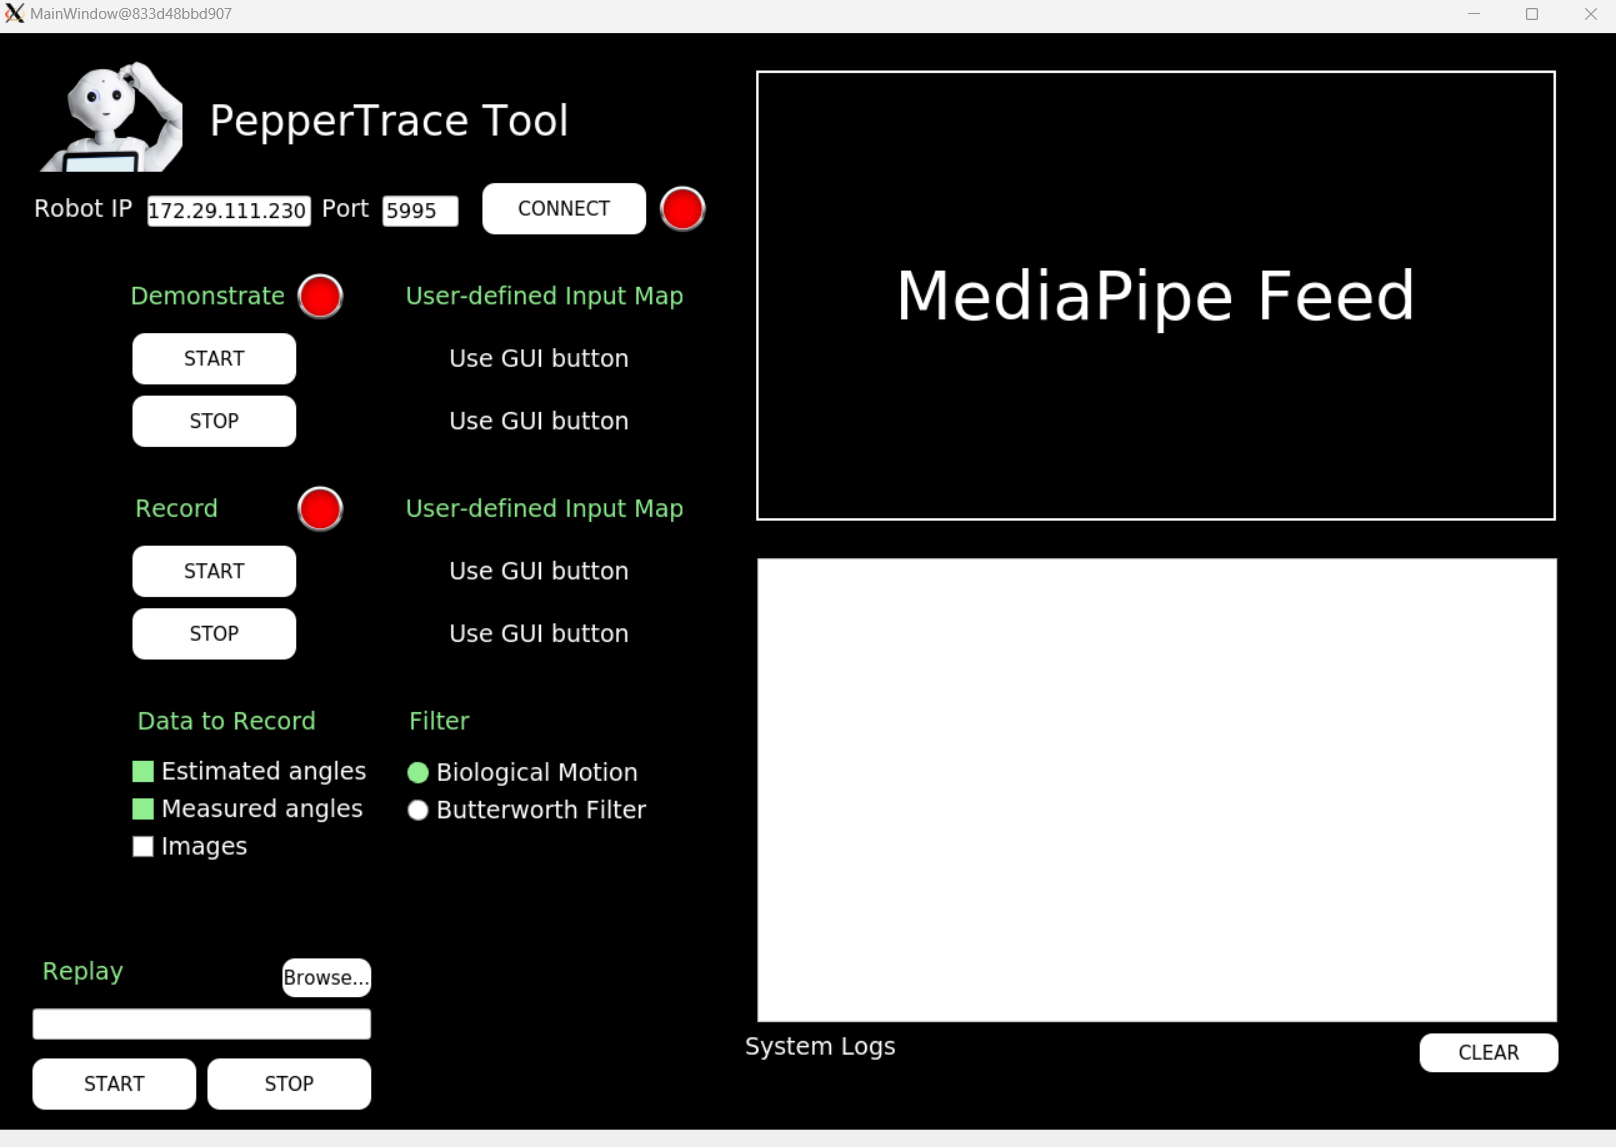
\includegraphics[width=\linewidth]{figures/peppertrace_gui.png}
    \caption{Graphical User Interface for the PepperTrace Programming by Demonstration Tool}
    \label{fig:gui}
\end{figure}
    
\newpage

\subsection{(Optional) Configuration}
The \texttt{programming\_by\_demonstration} software package consists of three components, \texttt{skeletal\_model}, \texttt{demonstration\_recorder} and \texttt{demonstration\_gui}, each with configuration files in their \texttt{/config} folders. 

\begin{description}
    
    \item[Configure skeletal model:] Besides the camera intrinsics there are other configuration options in the config file of the \texttt{skeletal\_model} component, however it is not necessary to change them. 
        
    \item[Configure demonstration recorder: ] You can check and  configure where data recordings are stored in the configuration file of the \texttt{demonstration\_recorder} component through the \texttt{data\_dir} (base directory) and \texttt{demo\_name} (demo directory) parameters. It is not necessary to change the parameters.

    \item[Configure demonstration gui: ] You can configure some parameters for the GUI in the configuration file of the \texttt{demonstration\_gui} component. This is not necessary. 
       
    
\end{description}



\newpage

\section{Main Features}

The PepperTrace GUI contains the following features for connecting to the robot, performing, recording and replaying demonstrations while logging imporant information for the user. 

\begin{description}
	\item[Connect: ] Enter the IP address and port of the Pepper robot and click the CONNECT button. This should connect the GUI to the Pepper robot and enable its controllers. Pressing the button again will stop the controllers and disconnect the robot.
    \item[Demonstrate: ] Press START under Demonstrate to enable demonstration. If a human is present in front of the camera, the software will capture its upper body movements and retarget them to Pepper in real time. Pressing STOP will stop this process.
	\item[Record: ] Press START under Record to record a demonstration. Check the boxes corresponding to the data that should be recorded during the demonstration. Demonstrate needs to be enabled for this to work. This will save the specified data to .bag files. 
	\item[Replay: ] Enter the path to a .bag file for replaying data and reproducing movement demonstrated in a previous recording session. Alternatively, click the Browse button and select the .bag file from the file dialog that appears. Click START to replay the bag file. The process will stop automatically when there is no more data to publish, unless you press STOP to before that. 
	\item[Logging: ] System logs (Infos, Warnings, Errors) are displayed to the System Logs box in the GUI. The skeletal model feed is displayed in the GUI when Demonstrate is on and the upper body joints of a human are detected in front of the camera. 
\end{description}

These features are illustrated in the behavioural graph in \cref{fig:behavioural}.

\begin{figure}[H]
    \centering
    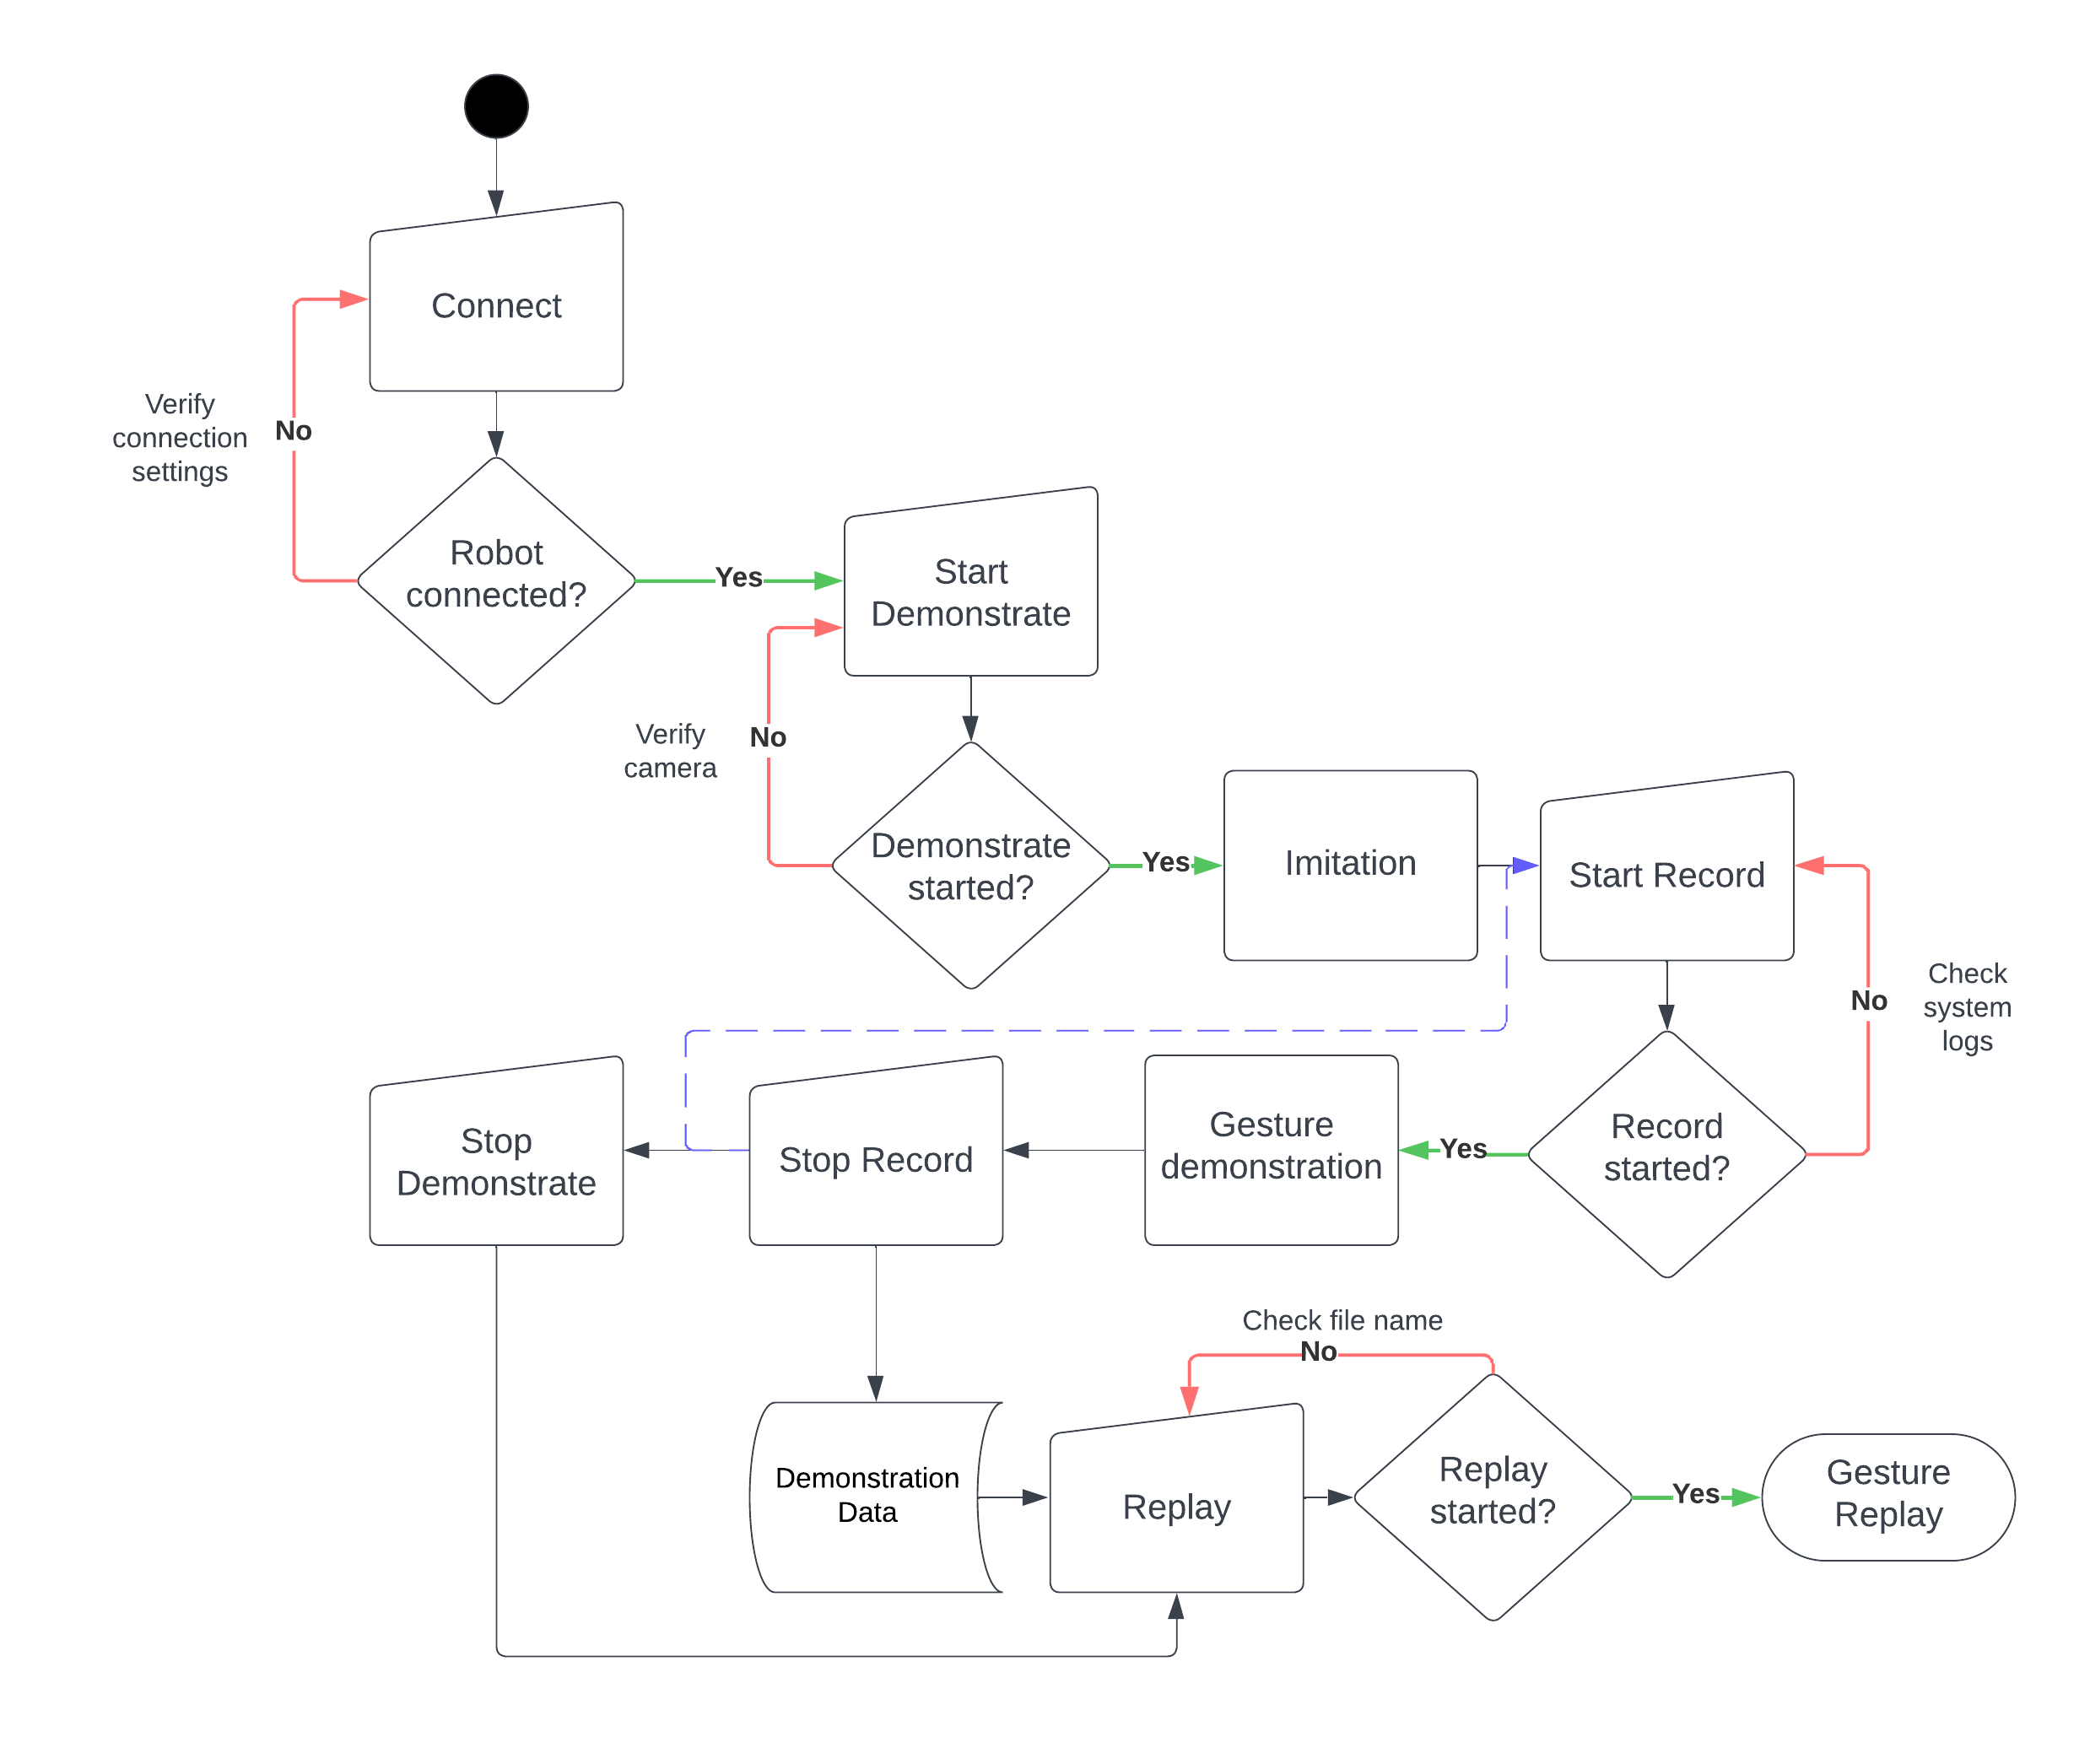
\includegraphics[width=\linewidth]{figures/BehaviouralGraph.png}
    \caption{Behavioural graph of the PbD module: The user-centered graph shows an example procedure for demonstrating, recording and replaying. Rectangular boxes represent observable processes, diamond-shaped boxes stand for checks, non-rectangular boxes represent user action. ``Gesture Replay" is the termination element. The blue line indicates the available option of recording multiple demonstrations in one session.}
    \label{fig:behavioural}
\end{figure}

\newpage

\section{Guidelines for Reporting Issues} \label{sec:report}
%===============================================================
To report an issue or request a feature, please follow these steps:

\begin{description}
    \item[Step 1:] Go to the \href{https://github.com/danielcortezbarros/peppertrace}{Github repository} and go to ``Issues".

    \item[Step 2:] Check if your issue exists, otherwise open a new issue by clicking ``New issue".

    \item[Step 3:] Add a label to the issue:
    \begin{description}
        \item[bug:] For reporting something that is not working.
        \item[new\_feature:] For requesting a new feature.
        \item[docs:] For requesting further documentation.
        \item[question:] For general remarks.
    \end{description}

    \item[Step 4:] Please give a descriptive title and report the issue as clearly and with as much detail as possible, including code sections if applicable.

    \item[Step 5:] Follow and monitor the issue, as the developers may have follow-ups.
\end{description}



%\newpage
%\bibliographystyle{unsrt}
%================================================================
%\bibliography{cognitive_systems.bib}                                     % REPLACE with correct filename
%\addcontentsline{toc}{section}{References}



\pagebreak
\section*{Principal Contributors}
%===============================================================
\label{contributors}
\addcontentsline{toc}{section}{Principal Contributors}
The main authors of this deliverable are as follows (in alphabetical order).
\blank
~
\blank
Daniel Barros, Carnegie Mellon University Africa.\\    % REPLACE with correct name and affiliation
David Vernon, Carnegie Mellon University Africa.\\    % REPLACE with correct name and affiliation                                                                  % REMOVE
 

  

\newpage
\section*{Document History}
%================================================================
\addcontentsline{toc}{section}{Document History}
\label{document_history}

\begin{description}

\item [Version 1.0]~\\
First draft. \\
Daniel Barros. \\                                     % REPLACE with correct name
2 December 2024.                                                        % REPLACE with correct date

\item [Version 1.1]~\\
Changed execution command to start an existing Docker container instead of creating a new one each time. \\
Daniel Barros. \\                                     % REPLACE with correct name
14 December 2024.                                                        % REPLACE with correct date

\item [Version 1.2]~\\
Formatting fixes, added suggestion to copy the commands from the Github repository's README.md file. Removed empty references page. \\
Daniel Barros. \\                                     % REPLACE with correct name
16 December 2024.                                                        % REPLACE with correct date


\end{description}

\end{document}

